%
% 31-ring.tex -- Funktionen auf einem Ringgebiet
%
% (c) 2026 Prof Dr Andreas Müller
%
\subsection{Funktionen auf einem Ringgebiet}
%
% fig-ring.tex
%
% (c) 2026 Prof Dr Andreas Müller
%
\begin{figure}
\centering
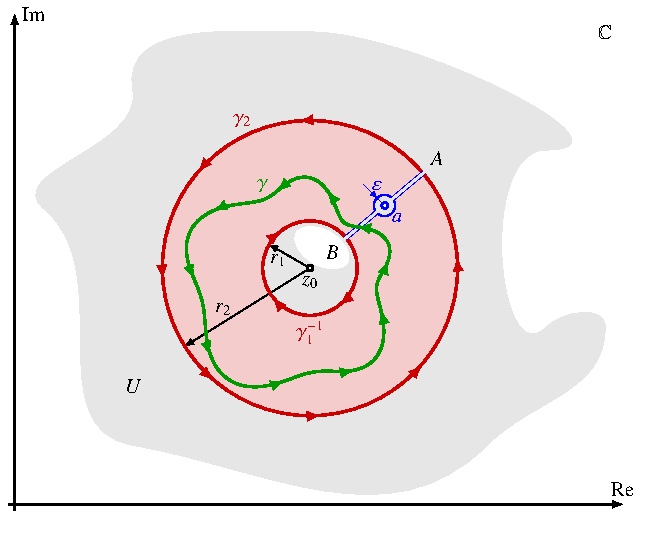
\includegraphics{chapters/040-analytisch/images/ring.pdf}
\caption{Die Funktion $f\colon U\to\mathbb{C}$ kann mithilfe eines
Pfadintegrals über den roten Rand berechnet werden, wodurch sich
die Entwicklung der Funktion in eine Laurent-Reihe finden lässt.
Die Koeffizienten der Laurent-Reihe können aber auch mit dem 
Weg $\gamma$ berechnet werden, der sich im Ringgebiet zu $\gamma_1$
oder $\gamma_2$ deformieren lässt.
\label{buch:analytisch:laurent:fig:ring}}
\end{figure}
%
Wir betrachten eine holomorphe Funktion $f\colon U\to\mathbb{C}$.
Die offene Menge $U$ sei so gestaltet, dass der \emph{Ring}
\[
R(z_0;r_1,r_2)
=
\{
z\in\mathbb{C}
\mid
r_1 \le |z-z_0| \le r_2
\}
\]
in $U$ enthalten ist.
\index{Ringgebiet}%
Abbildung~\ref{buch:analytisch:laurent:fig:ring} zeigt diese Situation.
Das Innere des Rings, der kleine Kreis mit Radius $r_1$ heisst auch
das \emph{Auge} des Rings.
\index{Auge}%

Da die Funktion $f$ im Inneren des kleinen Kreises mit Radius $r_1$ um
den Punkt $z_0$ nicht überall definiert sein muss, ist der Integralsatz
von Cauchy nicht auf den grossen Kreis anwendbar.
Der folgende Satz zeigt, dass es aber trotzdem möglich ist, den Wert von
$f$ in einem beliebigen Punkt des Ringgebietes mit einem Wegintegral
zu berechnen.

\begin{satz}
Seien $\gamma_2$ und $\gamma_1$ die im Gegenuhrzeigersinn durchlaufenen
Randkreise des Ringgebietes $R(z_0;r_1,r_2)$ mit Radien $r_2$ und $r_1$.
Dann gilt
\begin{equation}
f(a)
=
\frac{1}{2\pi i}
\oint_{\gamma_2}
\frac{f(z)}{z-a}
\,dz
-
\frac{1}{2\pi i}
\oint_{\gamma_1}
\frac{f(z)}{z-a}
\,dz
\label{buch:analytisch:laurent:eqn:zweiintegrale}
\end{equation}
für jeden Punkt $a\in R(z_0;r_1,r_2)$.
\end{satz}

\begin{proof}
Der in Abbildung~\ref{buch:analytisch:laurent:fig:ring} dargestellte
Weg, der vom Punkt $A$ ausgehend zunächst dem äusseren Randkreis
folgt bis wieder zurück zum Punkt $A$, dann radial zum Punkt $a$,
in einem Halbkreis vom Radius $\varepsilon$ um den Punkt $a$ und
dann geradlinig weiter bis zum Punkt $B$, von dort im Uhrzeigersinn
um den inneren Randkreis zurück zum Punkt $B$ und erneut radial zum
Punkt $A$, wieder mit einem kleinen, kreisförmigen Umweg vom Radius
$\varepsilon$ um den Punkt $a$.
Die Funktion ist im Inneren des Weges überall holomorph,
nach dem Integralsatz von Cauchy verschwindet das Integral über
den ganzen Weg.

Die radialen Teile werden zweimal in entgegengesetzter Richtung durchlaufen
und heben sich daher weg.
Somit bleiben nur noch die Integrale über die Teile $\gamma_2$,
$\gamma_1^{-1}$ und $\gamma_\varepsilon$, die zusammen das Integral
über die Kette $\gamma_2+\gamma_1^{-1}+\gamma_{\varepsilon}^{-1}$ mit
dem Wert
\[
0
=
\oint_{\gamma_2 + \gamma_1^{-1} + \gamma_{\varepsilon}^{-1}}
\frac{f(z)}{z-a}\,dz 
=
\oint_{\gamma_2}
\frac{f(z)}{z-a}\,dz 
-
\oint_{\gamma_1}
\frac{f(z)}{z-a}\,dz 
-
\oint_{\gamma_{\varepsilon}}
\frac{f(z)}{z-a}\,dz 
\]
ergeben.

Der kleine Kreis $\gamma_\varepsilon$ um den Punkt $a$ kann mit
$t\mapsto \varepsilon e^{2\pi it}$ parametrisiert werden, um das
Integral zu berechnen.
So wird aus dem Integral
\begin{align*}
0
&=
\oint_{\gamma_2} \frac{f(z)}{z-a}\,dz
-
\oint_{\gamma_1} \frac{f(z)}{z-a}\,dz
-
\int_0^1
\frac{f(a+\varepsilon e^{2\pi it})}{a+\varepsilon e^{2\pi it}-a}
\cdot
\frac{d}{dt}
\varepsilon
e^{2\pi it}
\,dt
\intertext{aufgelöst nach dem Integral über $\gamma_\varepsilon$}
\oint_{\gamma_2} \frac{f(z)}{z-a}\,dz
-
\oint_{\gamma_1} \frac{f(z)}{z-a}\,dz
&=
\int_0^1
\frac{f(a+\varepsilon e^{2\pi it})}{\varepsilon e^{2\pi it}}
\cdot
2\pi i\varepsilon e^{2\pi it}
\,dt
\\
&=
2\pi i
\int_0^1
f(a+\varepsilon e^{2\pi it})
\,dt.
\intertext{Das Integral auf der rechten Seite geht für $\varepsilon\to 0$
gegen $f(a)$, wir erhalten also}
&=
2\pi i f(a).
\intertext{Aufgelöst nach $f(a)$ finden wir}
f(a)
&=
\frac{1}{2\pi i}
\oint_{\gamma_2}
\frac{f(z)}{z-a}
\,dz
-
\frac{1}{2\pi i}
\oint_{\gamma_1}
\frac{f(z)}{z-a}
\,dz.
\end{align*}
Damit ist der Satz bewiesen.
\end{proof}

\begin{beispiel}
Wir betrachten die Funktion $f(z)=1/z$ im Ringgebiet $R(0;r_1,r_2)$ und
rechnen die Integralformel~\eqref{buch:analytisch:laurent:eqn:zweiintegrale}
nach.
Mit der Partialbruchzerlegung
\[
\frac{1}{z(z-a)}
=
\frac{1}{a}
\biggl(
\frac{1}{z}
+
\frac{1}{z-a}
\biggr)
\]
können die Integrale aufgespaltet und mit der Cauchy-Integralformel
berechnet werden als
\begin{align*}
\int_{\gamma_2} \frac{f(z)}{z-a}\,dz
&=
\frac1a
\int_{\gamma_2} {\color{darkred}\frac{1}{z}}+\frac{1}{z-a}\,dz
=
{\color{darkred}
\frac1a
\underbrace{
\int_{\gamma_2} \frac{1}{z}\,dz
}_{\displaystyle=2\pi i}
}
+
\frac1a
\underbrace{
\int_{\gamma_2}\frac{1}{z-a}\,dz
}_{\displaystyle=2\pi i}
%
\intertext{und}
\int_{\gamma_1} \frac{f(z)}{z-a}\,dz
&=
\frac1a
\int_{\gamma_1} {\color{darkred}\frac{1}{z}}+\frac{1}{z-a}\,dz
=
{\color{darkred}
\frac1a
\underbrace{
\int_{\gamma_1} \frac{1}{z}\,dz
}_{\displaystyle=2\pi i}
}
+
\frac1a
\underbrace{
\int_{\gamma_1} \frac{1}{z-a}\,dz.
}_{\displaystyle=0}
\end{align*}
Das letzte Integral verschwindet, weil die Funktion $1/(z-a)$ holomorph
ist im Auge des Ringgebietes.
Die Integralformel~\eqref{buch:analytisch:laurent:eqn:zweiintegrale}
wird jetzt zu
\begin{align*}
\frac{1}{2\pi i}
\int_{\gamma_2} \frac{f(z)}{z-a}\,dz
-
\frac{1}{2\pi i}
\int_{\gamma_1} \frac{f(z)}{z-a}\,dz
&=
{\color{darkred}\frac1a} + \frac1a - {\color{darkred}\frac1a}
=
\frac1a
=
f(a).
\end{align*}
Die Integralformel~\eqref{buch:analytisch:laurent:eqn:zweiintegrale}
berechnet tatsächlich den Funktionswert an der Stelle $a$.

Die roten Integrale sind Beiträge der Polstelle im Zentrum des Ringgebietes.
Da sie in beiden Integralen über $\gamma_2$ und $\gamma_1$ auftreten,
heben Sie sich in der Differenz weg, so dass nur noch der Beitrag
der Polstelle des Integranden bei $a$ übrig bleibt.
\end{beispiel}
